\documentclass[12pt]{article}

% Computational Physics by M. Newman
% Setup file for exercises

% Packages
\usepackage{mathpazo}
\usepackage{amsmath}
\usepackage{graphicx}
\usepackage{calrsfs}
\usepackage{fancyvrb}

% Formatting
\setlength{\textwidth}{17.5cm}
\setlength{\textheight}{24.0cm}
\setlength{\evensidemargin}{2.5cm}
\setlength{\oddsidemargin}{-0.6cm}
\setlength{\topmargin}{-2.3cm}
\setlength{\textfloatsep}{0pt}
\setcounter{secnumdepth}{0}
\renewcommand{\baselinestretch}{1.06}

% Macros
\newcommand{\dd}{\mathrm{d}}
\newcommand{\ii}{\mathrm{i}}
\newcommand{\e}{\mathrm{e}}
\newcommand{\half}{\tfrac12}
\newcommand{\av}[1]{\langle#1\rangle}
\newcommand{\var}{\mathop\mathrm{var}}
\newcommand{\Ord}{\mathrm{O}}
\renewcommand{\Re}{\mathop\mathrm{Re}\nolimits}
\renewcommand{\Im}{\mathop\mathrm{Im}\nolimits}
\newcommand{\mat}{\mathbf}
\renewcommand{\vec}{\mathbf}
\newcommand{\defn}{\textit}
\newcommand{\exskip}{\nopagebreak\medskip\noindent}
\newcommand{\pmstrut}{\rule{0pt}{13pt}}

% Environments
\newcounter{chapter}
\setcounter{chapter}{2}
\newcounter{exercise}
\renewcommand{\theexercise}{\arabic{chapter}.\arabic{exercise}}
\newenvironment{exercises}{\vspace{2ex plus0.5ex minus0.5ex}
  \renewcommand{\labelenumi}{\alph{enumi})}}%
    {\par\vspace{1ex plus0.5ex minus0.5ex}}
\newcommand{\exercise}{\refstepcounter{exercise}%
  \par\vspace{4ex plus1ex minus1ex}%
  \noindent\textbf{Exercise \theexercise: }}

\DefineVerbatimEnvironment{code}{Verbatim}{xleftmargin=\parindent}

\setcounter{chapter}{9}

\begin{document}

\noindent {\LARGE\textsc{Computational Physics}}\par
\bigskip
\noindent {\large\textsc{Exercises for Chapter \arabic{chapter}}}\par
\noindent\hrulefill

%%%%%%%%%%%%%%%%%%%%%%%%%%%%%%%%%%%%%%%%%%%%%%%%%%%%%%%%%%%%%%%%%%%%%%
%%%                                                                %%%
%%%     COMPUTATIONAL PHYSICS, M. NEWMAN, CHAPTER 9, EXERCISES     %%%
%%%                                                                %%%
%%%%%%%%%%%%%%%%%%%%%%%%%%%%%%%%%%%%%%%%%%%%%%%%%%%%%%%%%%%%%%%%%%%%%%

\begin{exercises}

%%% Exercise 9.1 %%%

\exercise Write a program, or modify the one from Example~9.1, to solve
  Poisson's equation for the system described in Example~9.2.  Work in
  units where $\epsilon_0=1$ and continue the iteration until your solution
  for the electric potential changes by less than $10^{-6}\,$V per step at
  every grid point.


%%% Exercise 9.2 %%%

\exercise Use the Gauss--Seidel method to solve Laplace's equation for
  the two-dimensional problem in Example~9.1---a square box $1\,$m on each
  side, at voltage~$V=1$ volt along the top wall and zero volts along the
  other three.  Use a grid of spacing $a=1\,$cm, so that there are 100 grid
  points along each wall, or 101 if you count the points at both ends.
  Continue the iteration of the method until the value of the electric
  potential changes by no more than $\delta=10^{-6}\,$V at any grid point
  on any step, then make a density plot of the final solution, similar to
  that shown in Fig.~9.3.  Experiment with different values of~$\omega$ to
  find which value gives the fastest solution.  As mentioned above, you
  should find that a value around 0.9 does well.  In general larger values
  cause the calculation to run faster, but if you choose too large a value
  the speed drops off and for values above 1 the calculation becomes
  unstable.

%%% Exercise 9.3 %%%

\exercise Consider the following simple model of an electronic capacitor,
consisting of two flat metal plates enclosed in a square metal box:
\medskip
\begin{center}
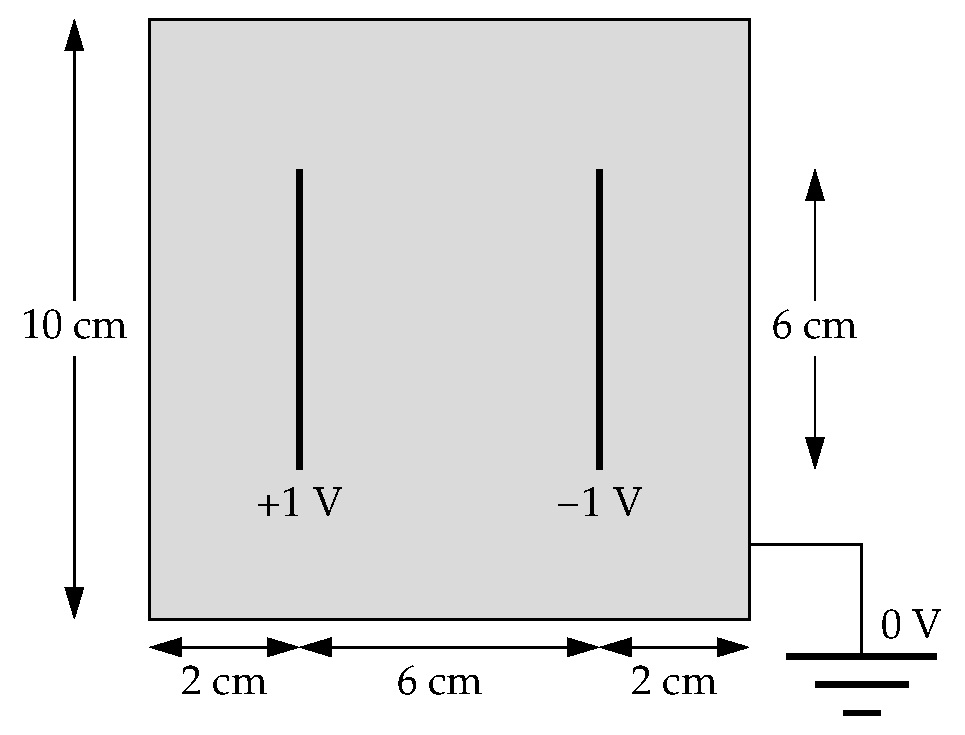
\includegraphics[width=9cm]{capacitor.eps}
\end{center}
For simplicity let us model the system in two dimensions.  Using any of the
methods we have studied, write a program to calculate the electrostatic
potential in the box on a grid of $100\times100$ points, where the walls of
the box are at voltage zero and the two plates (which are of negligible
thickness) are at voltages~$\pm1\,$V as shown.  Have your program calculate
the value of the potential at each grid point to a precision of
$10^{-6}\,$volts and then make a density plot of the result.

Hint: Notice that the capacitor plates are at fixed \emph{voltage}, not
fixed charge, so this problem differs from the problem with the two charges
in Exercise~9.1.  In effect, the capacitor plates are part of the boundary
condition in this case: they behave the same way as the walls of the box,
with potentials that are fixed at a certain value and cannot change.


%%% Exercise 9.4 %%%

\exercise \textbf{Thermal diffusion in the Earth's crust}

\exskip A classic example of a diffusion problem with a time-varying
boundary condition is the diffusion of heat into the crust of the Earth, as
surface temperature varies with the seasons.  Suppose the mean daily
temperature at a particular point on the surface varies as:
\begin{displaymath}
T_0(t) = A + B\sin {2\pi t\over\tau},
\end{displaymath}
where $\tau=365\,$days, $A=10^\circ$C and $B=12^\circ$C.  At a depth of
$20\,$m below the surface almost all annual temperature variation is ironed
out and the temperature is, to a good approximation, a constant $11^\circ$C
(which is higher than the mean surface temperature of
$10^\circ$C---temperature increases with depth, due to heating from the hot
core of the planet).  The thermal diffusivity of the Earth's crust
varies somewhat from place to place, but for our purposes we will treat it
as constant with value $D=0.1\,\mathrm{m}^2\,\mathrm{day}^{-1}$.

Write a program, or modify one of the ones given in this chapter, to
calculate the temperature profile of the crust as a function of depth up to
$20\,$m and time up to 10 years.  Start with temperature everywhere equal
to $10^\circ$C, except at the surface and the deepest point, choose values
for the number of grid points and the time-step~$h$, then run your program
for the first nine simulated years, to allow it to settle down into
whatever pattern it reaches.  Then for the tenth and final year plot four
temperature profiles taken at 3-month intervals on a single graph to
illustrate how the temperature changes as a function of depth and time.


%%% Exercise 9.5 %%%

\exercise \textbf{FTCS solution of the wave equation}

\exskip Consider a piano string of
length~$L$, initially at rest.  At time $t=0$ the string is struck by the
piano hammer a distance~$d$ from the end of the string:
\bigskip
\begin{center}
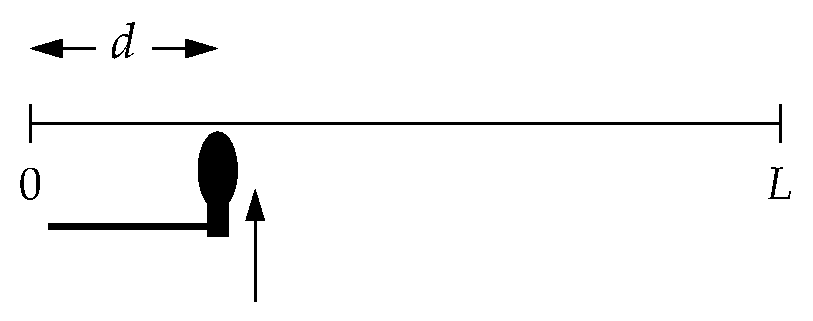
\includegraphics[width=7.5cm]{piano.eps}
\end{center}
\bigskip The string vibrates as a result of being struck, except at
the ends, $x=0$ and $x=L$, where it is held fixed.
\begin{enumerate}\setlength{\itemsep}{0pt}
\item Write a program that uses the FTCS method to solve the complete set
  of simultaneous first-order equations, Eq.~(9.28), for the case
  $v=100\,\mathrm{ms}^{-1}$, with the initial condition that $\phi(x)=0$
  everywhere but the velocity~$\psi(x)$ is nonzero, with profile
\begin{displaymath}
\psi(x) = C {x(L-x)\over L^2} \exp \biggl[ -{(x-d)^2\over2\sigma^2} \biggr],
\end{displaymath}
where $L=1\,$m, $d=10\,$cm, $C=1\,\mathrm{ms}^{-1}$, and $\sigma=0.3\,$m.
You will also need to choose a value for the time-step~$h$.  A reasonable
choice is $h=10^{-6}\,$s.
\item Make an animation of the motion of the piano string using the
  facilities provided by the \verb|visual| package, which we studied in
  Section~3.4.  There are various ways you could do this.  A simple one
  would be to just place a small sphere at the location of each grid point
  on the string.  A more sophisticated approach would be to use the
  \verb|curve| object in the \verb|visual| package---see the on-line
  documentation at \texttt{www.vpython.org} for details.  A convenient
  feature of the curve object is that you can specify its set of $x$
  positions and $y$ positions separately as arrays.  In this exercise the
  $x$ positions only need to specified once, since they never change, while
  the $y$ positions will need to be specified anew each time you take a
  time-step.  Also, since the vertical displacement of the string is much
  less than its horizontal length, you will probably need to multiply the
  vertical displacement by a fairly large factor to make it visible on the
  screen.

  Allow your animation to run for some time, until numerical instabilities
  start to appear.
\end{enumerate}


%%% Exercise 9.6 %%%

\exercise What would the equivalent of Eq.~(9.7) be in three dimensions?


%%% Exercise 9.7 %%%

\exercise \textbf{The relaxation method for ordinary differential
  equations}

\exskip There is no reason why the relaxation method must be restricted to
the solution of differential equations with two or more independent
variables.  It can also be applied to those with one independent variable,
i.e.,~to ordinary differential equations.  In this context, as with partial
differential equations, it is a technique for solving boundary value
problems, which are less common with ordinary differential equations but do
occur---we discussed them in Section~8.6.

Consider the problem we looked at in Example~8.8 on page~390, in which a
ball of mass $m=1\,$kg is thrown from height $x=0$ into the air and lands
back at $x=0$ ten seconds later.  The problem is to calculate the
trajectory of the ball, but we cannot do it using initial value methods
like the ordinary Runge--Kutta method because we are not told the initial
velocity of the ball.  One approach to finding a solution is the shooting
method of Section~8.6.1.  Another is the relaxation method.

Ignoring friction effects, the trajectory is the solution of the ordinary
differential equation
\begin{displaymath}
{\dd^2 x\over\dd t^2} = -g,
\end{displaymath}
where $g$ is the acceleration due to gravity.
\begin{enumerate}\setlength{\itemsep}{0pt}
\item Replacing the second derivative in this equation with its
  finite-difference approximation, Eq.~(5.109), derive a relaxation-method
  equation for solving this problem on a time-like ``grid'' of points with
  separation~$h$.
\item Taking the boundary conditions to be that $x=0$ at $t=0$ and $t=10$,
  write a program to solve for the height of the ball as a function of time
  using the relaxation method with 100 points and make a plot of the result
  from $t=0$ to $t=10$.  Run the relaxation method until the answers change
  by $10^{-6}$ or less at every point on each step.
\end{enumerate}
Note that, unlike the shooting method, the relaxation method does not give
us the initial value of the velocity needed to achieve the required
solution.  It gives us only the solution itself, although one could get an
approximation to the initial velocity by calculating a numerical derivative
of the solution at time~$t=0$.  On balance, however, the relaxation method
for ordinary differential equations is most useful when one wants to know
the details of the solution itself, but not the initial conditions needed
to achieve~it.



%%% Exercise 9.8 %%%

\exercise \textbf{The Schr\"odinger equation and the Crank--Nicolson
  method}

\exskip Perhaps the most important partial differential equation, at least
for physicists, is the Schr\"odinger equation.  This exercise uses the
Crank--Nicolson method to solve the full time-dependent Schr\"odinger
equation and hence develop a picture of how a wavefunction evolves over
time.  The following exercise, Exercise~9.9, solves the same problem again,
but using the spectral method.

We will look at the Schr\"odinger equation in one dimension.  The
techniques for calculating solutions in two or three dimensions are
basically the same as for one dimension, but the calculations take much
longer on the computer, so in the interests of speed we'll stick with one
dimension.  In one dimension the Schr\"odinger equation for a particle of
mass~$M$ with no potential energy reads
\begin{displaymath}
-{\hbar^2\over2M} {\partial^2\psi\over\partial x^2}
  = \ii\hbar {\partial\psi\over\partial t}.
\end{displaymath}
For simplicity, let's put our particle in a box with impenetrable
walls, so that we only have to solve the equation in a finite-sized space.
The box forces the wavefunction~$\psi$ to be zero at the walls, which we'll
put at $x=0$ and $x=L$.

Replacing the second derivative in the Schr\"odinger equation with a
finite difference and applying Euler's method, we get the FTCS equation
\begin{displaymath}
\psi(x,t+h) = \psi(x,t) + h {\ii\hbar\over2ma^2} \bigl[ \psi(x+a,t)
              + \psi(x-a,t) - 2\psi(x,t) \bigr],
\end{displaymath}
where $a$ is the spacing of the spatial grid points and $h$ is the size of
the time-step.  (Be careful not to confuse the time-step~$h$ with Planck's
constant~$\hbar$.)  Performing a similar step in reverse, we get the
implicit equation
\begin{displaymath}
\psi(x,t+h) - h {\ii\hbar\over2ma^2} \bigl[ \psi(x+a,t+h)
              + \psi(x-a,t+h) - 2\psi(x,t+h) \bigr] = \psi(x,t).
\end{displaymath}
And taking the average of these two, we get the Crank--Nicolson equation
for the Schr\"odinger equation:
\begin{align*}
\psi(x,t+h) - h {\ii\hbar\over4ma^2} \bigl[ &\psi(x+a,t+h)
              + \psi(x-a,t+h) - 2\psi(x,t+h) \bigr] \nonumber\\
  &= \psi(x,t) + h {\ii\hbar\over4ma^2} \bigl[ \psi(x+a,t)
              + \psi(x-a,t) - 2\psi(x,t) \bigr].
\end{align*}
This gives us a set of simultaneous equations, one for each grid point.

The boundary conditions on our problem tell us that $\psi=0$ at
$x=0$ and $x=L$ for all~$t$.  In between these points we have grid points
at $a$, $2a$, $3a$, and so forth.  Let us arrange the values of~$\psi$ at
these interior points into a vector
\begin{displaymath}
\boldsymbol{\psi}(t)
  = \begin{pmatrix} \psi(a,t) \\ \psi(2a,t) \\ \psi(3a,t) \\ \vdots
    \end{pmatrix}.
\end{displaymath}
Then the Crank--Nicolson equations can be written in the form
\begin{displaymath}
\mat{A}\boldsymbol{\psi}(t+h) = \mat{B}\boldsymbol{\psi}(t),
\end{displaymath}
where the matrices $\mat{A}$ and~$\mat{B}$ are both symmetric and
tridiagonal:
\begin{displaymath}
\mat{A} = \begin{pmatrix} a_1 & a_2 \\
                          a_2 & a_1 & a_2 \\
                              & a_2 & a_1 & a_2 \\
                              &     & a_2 & a_1 \\
                              &     &     &     & \ddots
          \end{pmatrix},\qquad\qquad
\mat{B} = \begin{pmatrix} b_1 & b_2 \\
                          b_2 & b_1 & b_2 \\
                              & b_2 & b_1 & b_2 \\
                              &     & b_2 & b_1 \\
                              &     &     &     & \ddots
          \end{pmatrix},
\end{displaymath}
with
\begin{displaymath}
a_1 = 1 + h {\ii\hbar\over2ma^2},\qquad
a_2 = - h {\ii\hbar\over4ma^2},\qquad
b_1 = 1 - h {\ii\hbar\over2ma^2},\qquad
b_2 = h {\ii\hbar\over4ma^2}.
\end{displaymath}
(Note the different signs and the factors of 2 and 4 in the denominators.)

The equation $\mat{A}\boldsymbol{\psi}(t+h) = \mat{B}\boldsymbol{\psi}(t)$
has precisely the form $\mat{A}\vec{x} = \vec{v}$ of the simultaneous
equation problems we studied in Chapter~6 and can be solved using the same
methods.  Specifically, since the matrix~$\mat{A}$ is tridiagonal in this
case, we can use the fast tridiagonal version of Gaussian elimination that
we looked at in Section~6.1.6.

Consider an electron (mass $M=9.109\times10^{-31}\,$kg) in a box of
length~$L=10^{-8}\,$m.  Suppose that at time $t=0$ the wavefunction of the
electron has the form
\begin{displaymath}
\psi(x,0) = \exp \biggl[ -{(x-x_0)^2\over2\sigma^2} \biggr]
            \e^{\ii\kappa x},
\end{displaymath}
where
\begin{displaymath}
x_0 = {L\over2},\qquad
\sigma = 1\times10^{-10}\,\mathrm{m},\qquad
\kappa = 5\times10^{10}\,\mathrm{m}^{-1},
\end{displaymath}
and $\psi=0$ on the walls at $x=0$ and $x=L$.  (This expression for
$\psi(x,0)$ is not normalized---there should really be an overall
multiplying coefficient to make sure that the probability density for the
electron integrates to unity.  It's safe to drop the constant, however,
because the Schr\"odinger equation is linear, so the constant cancels out
on both sides of the equation and plays no part in the solution.)

\begin{enumerate}\setlength{\itemsep}{0pt}
\item Write a program to perform a single step of the
  Crank--Nicolson method for this electron, calculating the vector
  $\boldsymbol{\psi}(t)$ of values of the wavefunction, given the initial
  wavefunction above and using~$N=1000$ spatial slices with $a=L/N$.  Your
  program will have to perform the following steps.  First, given the
  vector $\boldsymbol{\psi}(0)$ at $t=0$, you will have to multiply by the
  matrix~$\mat{B}$ to get a vector~$\vec{v} = \mat{B}\boldsymbol{\psi}$.
  Because of the tridiagonal form of~$\mat{B}$, this is fairly simple.  The
  $i$th component of~$\vec{v}$ is given by
\begin{displaymath}
v_i = b_1\psi_i + b_2(\psi_{i+1}+\psi_{i-1}).
\end{displaymath}
You will also have to choose a value for the time-step~$h$.  A reasonable
choice is $h=10^{-18}\,$s.

Second you will have to solve the linear system $\mat{A}\mat{x}=\vec{v}$
for~$\vec{x}$, which gives you the new value of~$\boldsymbol{\psi}$.  You
could do this using a standard linear equation solver like the function
\verb|solve| in \verb|numpy.linalg|, but since the matrix~$\mat{A}$ is
tridiagonal a better approach would be to use the fast solver for banded
matrices given in Appendix~E, which can be imported from the file
\verb|banded.py| (which you can find in the on-line resources).  This solver works fine with complex-valued arrays, which you'll need to use to represent the wavefunction~$\boldsymbol{\psi}$ and the matrix~$\mat{A}$.

Third, once you have the code in place to perform a single step of the
calculation, extend your program to perform repeated steps and hence solve
for $\psi$ at a sequence of times a separation~$h$ apart.  Note that the
matrix~$\mat{A}$ is independent of time, so it doesn't change from one step
to another.  You can set up the matrix just once and then keep on reusing
it for every step.

\item Extend your program to make an animation of the solution by
  displaying the real part of the wavefunction at each time-step.  You can
  use the function \verb|rate| from the package \verb|visual| to ensure a
  smooth frame-rate for your animation---see Section~3.5 on page~117.

  There are various ways you could do the animation.  A simple one would be
  to just place a small sphere at each grid point with vertical position
  representing the value of the real part of the wavefunction.  A more
  sophisticated approach would be to use the \verb|curve| object
  from the \verb|visual| package---see the on-line documentation at
  \texttt{www.vpython.org} for details.  Depending on what coordinates you
  use for measuring~$x$, you may need to scale the values of the
  wavefunction by an additional constant to make them a reasonable size on
  the screen.  (If you measure your $x$ position in meters then a scale
  factor of about $10^{-9}$ works well for the wavefunction.)

\item Run your animation for a while and describe what you see.  Write a
  few sentences explaining in physics terms what is going on in the system.
\end{enumerate}



%%% Exercise 9.9 %%%

\exercise \textbf{The Schr\"odinger equation and the spectral method}

\exskip This exercise uses the spectral method to solve the time-dependent
Sch\"odinger equation
\begin{displaymath}
-{\hbar^2\over2M} {\partial^2\psi\over\partial x^2}
  = \ii\hbar {\partial\psi\over\partial t}
\end{displaymath}
for the same system as in Exercise~9.8, a single particle in one dimension
in a box of length~$L$ with impenetrable walls.  The wavefunction in such a
box necessarily goes to zero on the walls and hence one possible
(unnormalized) solution of the equation is
\begin{displaymath}
\psi_k(x,t) = \sin \biggl( {\pi k x\over L} \biggr)\,\e^{\ii Et/\hbar},
\end{displaymath}
where the energy~$E$ can be found by substituting into the Schr\"odinger
equation, giving
\begin{displaymath}
E = {\pi^2\hbar^2k^2\over2ML^2}.
\end{displaymath}
As with the vibrating string of Section~9.3.4, we can write a full solution
as a linear combination of such individual solutions, which on the grid
points $x_n=nL/N$ takes the value
\begin{displaymath}
\psi(x_n,t) = {1\over N}
              \sum_{k=1}^{N-1} b_k \sin \biggl( {\pi k n\over N} \biggr)\>
              \exp \biggl( \ii{\pi^2\hbar k^2\over2ML^2} t \biggr),
\end{displaymath}
where the $b_k$ are some set of (possibly complex) coefficients that
specify the exact shape of the wavefunction and the leading factor of $1/N$
is optional but convenient.

Since the Schr\"odinger equation (unlike the wave equation) is first order
in time, we need only a single initial condition on the value
of~$\psi(x,t)$ to specify the coefficients~$b_k$, although, since the
coefficients are in general complex, we will need to calculate both real
and imaginary parts of each coefficient.

As in Exercise~9.8 we consider an electron (mass
$M=9.109\times10^{-31}\,$kg) in a box of length~$L=10^{-8}\,$m.  At time
$t=0$ the wavefunction of the electron has the form
\begin{displaymath}
\psi(x,0) = \exp \biggl[ -{(x-x_0)^2\over2\sigma^2} \biggr]
            \e^{\ii\kappa x},
\end{displaymath}
where
\begin{displaymath}
x_0 = {L\over2},\qquad
\sigma = 1\times10^{-10}\,\mathrm{m},\qquad
\kappa = 5\times10^{10}\,\mathrm{m}^{-1},
\end{displaymath}
and $\psi=0$ on the walls at $x=0$ and $x=L$.

\begin{enumerate}\setlength{\itemsep}{0pt}
\item Write a program to calculate the values of the coefficients~$b_k$,
  which for convenience can be broken down into their real and imaginary
  parts as $b_k=\alpha_k+\ii\eta_k$.  Divide the box into $N=1000$ slices
  and create two arrays containing the real and imaginary parts of
  $\psi(x_n,0)$ at each grid point.  Perform discrete sine
  transforms on each array separately and hence calculate the values of
  the~$\alpha_k$ and~$\eta_k$ for all~$k=1\ldots N-1$.

  To perform the discrete sine transforms, you can use the fast transform
  function \verb|dst| from the package \verb|dcst|, which you can find in
  the on-line resources in the file named \verb|dcst.py|.  A copy of the
  code for the package can also be found in Appendix~E.  The function takes
  an array of $N$ real numbers and returns the discrete sine transform as
  another array of~$N$ numbers.

  (Note that the first element of the input array should in principle
  always be zero for a sine transform, but if it is not the \Verb|dst|
  function will simply pretend that it is.  Similarly the first element of
  the returned array is always zero, since the $k=0$ coefficient of a sine
  transform is always zero.  So in effect, the sine transform really only
  takes $N-1$ real numbers and transforms them into another $N-1$ real
  numbers.  In some implementations of the discrete sine transform,
  therefore, though not the one in the package \Verb|dsct| used here, the
  first element of each array is simply omitted, since it's always zero
  anyway, and the arrays are only $N-1$ elements long.)
\item Putting $b_k=\alpha_k+\ii\eta_k$ in the solution above and taking the
  real part we get
\begin{displaymath}
\Re \psi(x_n,t) = {1\over N} \sum_{k=1}^{N-1}
            \biggl[ \alpha_k \cos \biggl( {\pi^2\hbar k^2\over2ML^2} t \biggr)
            - \eta_k \sin \biggl( {\pi^2\hbar k^2\over2ML^2} t \biggr) \biggr]
            \sin \biggl( {\pi k n\over N} \biggr)
\end{displaymath}
for the real part of the wavefunction.  This is an inverse sine
transform with coefficients equal to the quantities in the square brackets.
Extend your program to calculate the real part of the
wavefunction~$\psi(x,t)$ at an arbitrary time~$t$ using this formula and
the inverse discrete sine transform function~\verb|idst|, also from the
package~\verb|dcst|.  Test your program by making a graph of the
wavefunction at time $t=10^{-16}\,$s.

\item Extend your program further to make an animation of the wavefunction
  over time, similar to that described in part~(b) of Exercise~9.8 above.
  A suitable time interval for each frame of the animation is about
  $10^{-18}\,$s.

\item Run your animation for a while and describe what you see.  Write a
  few sentences explaining in physics terms what is going on in the system.
\end{enumerate}

\end{exercises}

\end{document}
